%% Los índices de robustez premian las planificaciones nominales deficientes
%% Plantilla Elsevier CAS de una columna (cas-sc) — formato de envío
%% Revista objetivo: Computers & Industrial Engineering

\documentclass[a4paper,fleqn]{cas-sc}

\usepackage[authoryear,longnamesfirst]{natbib}
\usepackage{amsmath,amssymb,amsthm}
\usepackage{booktabs}
\usepackage{multirow}
\usepackage{graphicx}
\usepackage[spanish,es-noquoting]{babel}

\newtheorem{proposition}{Proposición}
\newtheorem{corollary}{Corolario}
\newdefinition{definition}{Definición}
\newproof{pf}{Demostración}

% Spanish labels for the CAS class
\AtBeginDocument{%
  \RenewDocumentCommand \printorcid { } { }%
}

\newcommand{\NRegimes}{9}
\newcommand{\NRunsDisrupted}{4{,}500}
\newcommand{\NInstances}{43}
\newcommand{\NConfRegimes}{6}
\newcommand{\NDescRegimes}{3}
\newcommand{\RhoConfMin}{\ensuremath{-0.985}}
\newcommand{\RhoConfMax}{\ensuremath{-0.948}}
\newcommand{\RhoConfMedian}{\ensuremath{-0.948}}
\newcommand{\PConfMax}{\ensuremath{3\times10^{-5}}}
\newcommand{\RhoDesc}{\ensuremath{-0.800}}
\newcommand{\NRhoNegative}{9}
\newcommand{\NDisagree}{9}
\newcommand{\PenaltyMin}{15.8}
\newcommand{\PenaltyMax}{49.3}
\newcommand{\PenaltyMedian}{25.7}
\newcommand{\TauMin}{\ensuremath{-0.60}}
\newcommand{\TauMax}{\ensuremath{-0.29}}
\newcommand{\NRLNotWorse}{9}
\newcommand{\NRLBest}{5}
\newcommand{\FriedmanPMax}{\ensuremath{6.7\times10^{-28}}}
\newcommand{\ArrCD}{0.79}
\newcommand{\ArrRankMin}{1.57}
\newcommand{\ArrRankMax}{1.62}
\newcommand{\ArrGapMin}{0.11}
\newcommand{\ArrGapMax}{0.20}
\newcommand{\CRWins}{6}
\newcommand{\LWKRWins}{3}
\newcommand{\CompGlobal}{233.4}
\newcommand{\CompFamily}{132.4}
\newcommand{\CompOracle}{7.6}
\newcommand{\CompPMax}{\ensuremath{4.1\times10^{-5}}}
\newcommand{\PropCells}{150}
\newcommand{\PropErr}{\ensuremath{9.4\times10^{-6}}}
\newcommand{\PctRINeg}{65}
\newcommand{\NRINeg}{97}
\newcommand{\QCpsat}{42.0}
\newcommand{\QGa}{41.3}
\newcommand{\QMor}{44.1}
\newcommand{\QMwkr}{46.8}
\newcommand{\QRl}{48.0}
\newcommand{\WallGa}{30}
\newcommand{\WallCpsat}{0.046}
\newcommand{\WallRl}{0.095}
\newcommand{\PRlCpsat}{0.375}
\newcommand{\PRlGa}{0.250}
\newcommand{\NEffOffline}{4}
\newcommand{\NExcludedArr}{5}
\newcommand{\CVaRTail}{3}
\newcommand{\SeedsPerCell}{30}
\newcommand{\CliqueArr}{1}
\newcommand{\CliqueOther}{3}
\newcommand{\NomRlTwo}{18.4}
\newcommand{\NomCrTwo}{220.1}
\newcommand{\NomRlAll}{24.8}
\newcommand{\NomCrAll}{430.3}
\newcommand{\NomMwkrTwo}{30.7}

\newcommand{\Cmax}{C_{\max}}
\newcommand{\RI}{\mathrm{RI}}
\newcommand{\RQ}{\mathrm{CR}}
\newcommand{\CVaR}{\mathrm{CVaR}}

\begin{document}
\let\WriteBookmarks\relax
\def\floatpagepagefraction{1}
\def\textpagefraction{.001}

\shorttitle{Los índices de robustez premian las planificaciones deficientes}
\shortauthors{J. J. Sánchez Acuña}

\title[mode=title]{Los índices de robustez premian las planificaciones
nominales deficientes: una auditoría de medición de la programación dinámica de
talleres bajo perturbación}

\author[1]{Joseph Javier Sánchez Acuña}
\cormark[1]
\ead{joseph.sanchez@uniminuto.edu.co}
\credit{Conceptualización, Metodología, Software, Análisis formal,
Investigación, Curación de datos, Redacción -- borrador original,
Redacción -- revisión y edición, Visualización}

\affiliation[1]{organization={Universidad de los Andes},
                city={Bogotá},
                country={Colombia}}

\cortext[1]{Autor de correspondencia.}

\begin{abstract}
El aprendizaje por refuerzo profundo (DRL) se propone cada vez con más
frecuencia para la programación dinámica de talleres bajo el argumento de que
las políticas de despacho aprendidas son más \emph{robustas} ante la
perturbación que la optimización fuera de línea. Esa afirmación se sostiene casi
siempre sobre un índice de robustez de la forma
$\RI=(\mathbb{E}[\Cmax^{\text{pert}}]-\Cmax^{\text{nom}})/\Cmax^{\text{nom}}$,
que normaliza la degradación que sufre un método por su propio makespan sin
perturbar. Mostramos, analítica y empíricamente, que esa normalización
autorreferencial vuelve el índice inservible para comparar métodos. Escribiendo
$r$ y $q$ para las desviaciones relativas del makespan nominal y del realizado
respecto de un óptimo certificado, demostramos que $\RI=(q-r)/(1+r)$, de modo
que a igual desempeño realizado $\RI$ es estrictamente decreciente en $r$:
cuanto peor es la planificación nominal de un método, más robusto parece. En un
corpus de \NRunsDisrupted{} ejecuciones perturbadas que abarca \NRegimes{}
regímenes preregistrados de tres clases de perturbación, $\RI$ correlaciona por
rangos de forma negativa con la desviación nominal en todos los regímenes, con
$\rho_s$ entre \RhoConfMin{} y \RhoConfMax{} ($p\le\PConfMax{}$) en los
\NConfRegimes{} regímenes que comparan diez métodos, y el orden que induce
discrepa del orden por calidad realizada en los \NRegimes{} ($\tau$ de Kendall
negativo sin excepción). Elegir un programador por $\RI$ en lugar de por calidad
realizada cuesta entre \PenaltyMin{} y \PenaltyMax{} puntos porcentuales de
desviación respecto del óptimo (mediana \PenaltyMedian{}). Proponemos la calidad
realizada --- la desviación del makespan ejecutado respecto del óptimo
certificado --- junto con su cola $\CVaR_{90}$, y una disciplina de reporte de
tres comparadores que separa la regla media, la mejor regla por familia y el
oráculo por instancia. Remedida así, una política PPO sobre red neuronal de
grafos heterogénea resulta estadísticamente indistinguible del mejor comparador
en los \NRegimes{} regímenes y ocupa el primer lugar en \NRLBest{}, incluidos los
tres de llegadas dinámicas: una conclusión que el índice convencional invierte.
\end{abstract}

\begin{highlights}
\item Se demuestra que el índice de robustez convencional es una función
estrictamente decreciente de la desviación nominal a desempeño realizado fijo.
\item Correlaciona con la desviación nominal en los nueve regímenes de
perturbación, con $\rho_s=-0{,}95$ a $-0{,}98$ donde se comparan diez métodos:
peores planificaciones nominales puntúan como más robustas.
\item El orden por el índice contradice el orden por calidad realizada en los
nueve regímenes, con un costo de hasta 49,3 puntos porcentuales.
\item La calidad realizada frente a un óptimo certificado, más una cola
$\CVaR_{90}$, restablece la comparabilidad entre métodos sin nuevos
experimentos.
\item Bajo la métrica corregida, una política GNN--PPO iguala al mejor
comparador en todos los regímenes y ocupa el primer lugar en cinco, incluidos
los de llegadas.
\end{highlights}

\begin{keywords}[Palabras clave]
Programación dinámica de talleres \sep Medición de robustez \sep
Aprendizaje por refuerzo profundo \sep Redes neuronales de grafos \sep
Programación con restricciones \sep Metodología experimental
\end{keywords}

\maketitle

% ===========================================================================
\section{Introducción}\label{sec:intro}

Las planificaciones de producción se calculan bajo supuestos que la planta no
respeta. Las máquinas fallan, los tiempos de proceso se realizan lejos de sus
estimaciones y llegan trabajos después de que la planificación quedó fijada. La
literatura ha respondido con dos estrategias amplias: calcular una planificación
fuera de línea y repararla conforme ocurren los eventos, o aprender una política
de despacho que decide en línea y que, por tanto, nunca se compromete con una
secuencia que después deba abandonar \citep{ouelhadj2009,aytug2005}. La segunda
ha concentrado un interés reciente intenso, con redes neuronales de grafos
aportando una representación de estado agnóstica al tamaño y métodos de
gradiente de política aportando la señal de aprendizaje
\citep{zhang2020,park2021,song2023,bengio2021}.

El argumento empírico a favor de las políticas aprendidas descansa sobre una
afirmación de robustez. Se sostiene que una política aprendida se degrada menos
bajo perturbación que un óptimo fuera de línea, y esto se cuantifica mediante un
índice que compara el makespan perturbado de un método con su propio makespan
sin perturbar:
\begin{equation}\label{eq:ri-intro}
  \RI \;=\; \frac{\mathbb{E}\!\left[\Cmax^{\text{pert}}\right]-\Cmax^{\text{nom}}}
                 {\Cmax^{\text{nom}}}.
\end{equation}
Variantes de \eqref{eq:ri-intro} aparecen a lo largo de la literatura de
programación robusta \citep{leon1994,mehta1998,goren2008,sabuncuoglu2000} y se
han trasladado a la literatura de programación con DRL en buena medida sin
examen \citep{smit2025,huang2025,xu2024survey}. El índice tiene una lectura
atractiva: es adimensional, es comparable entre instancias de distinto tamaño y
un valor cercano a cero dice que la perturbación le costó poco al método.

Este trabajo sostiene que \eqref{eq:ri-intro} no puede soportar el peso
comparativo que se le impone, y que el problema es estructural antes que una
cuestión de ruido de estimación. El denominador es el makespan nominal del
propio método. Un método que produce una planificación nominal deficiente queda
así calificado contra una referencia indulgente, y uno que produce una
planificación casi óptima, contra una exigente. La
Sección~\ref{sec:framework} lo hace exacto: con $r$ la desviación relativa del
makespan nominal respecto de un óptimo certificado y $q$ la desviación relativa
del makespan realizado respecto del mismo óptimo, $\RI=(q-r)/(1+r)$, cuya
derivada parcial en $r$ es estrictamente negativa. Dos métodos que entregan
planificaciones ejecutadas \emph{idénticas} quedan ordenados por $\RI$ en orden
inverso a la calidad de los planes de los que partieron.

La consecuencia no es hipotética. Reanalizamos un corpus preregistrado de
\NRunsDisrupted{} ejecuciones perturbadas que cubre tres clases de perturbación
a tres severidades cada una --- averías de máquina, tiempos de proceso
estocásticos y llegadas dinámicas de trabajos --- para nueve reglas de despacho
por prioridad y una política GNN--PPO heterogénea, junto con \NInstances{}
instancias nominales con óptimos probados. En cada uno de los \NRegimes{}
regímenes, $\RI$ correlaciona por rangos de forma negativa con cuán mala fue la
planificación nominal --- de manera casi perfecta en los \NConfRegimes{}
regímenes que comparan diez métodos --- y el método que nomina como más robusto
nunca es el que efectivamente termina más cerca del óptimo. Bajo averías y tiempos
estocásticos el índice corona a la regla de razón crítica, cuyas planificaciones
nominales se sitúan un $220\%$ por encima del óptimo; bajo llegadas dinámicas
corona a menor trabajo restante, con $187\%$. Ambas están entre los peores
desempeños una vez que la planificación ejecutada se mide contra una referencia
fija.

\paragraph{Contribuciones.} Este trabajo hace cuatro.
\begin{enumerate}[(i)]
\item \textbf{Una caracterización analítica del modo de falla.} La
Proposición~\ref{prop:ri} descompone $\RI$ en desviación nominal y realizada y
muestra la dependencia monótona de la primera; el
Corolario~\ref{cor:neg} identifica el $\RI$ negativo --- reportado
rutinariamente como robustez elevada --- como la firma de una planificación
nominal tan deficiente que la perturbación la mejora en esperanza.
\item \textbf{Una cuantificación del error de decisión resultante.} En los
\NRegimes{} regímenes, el orden por $\RI$ y el orden por calidad realizada
discrepan sin excepción, y actuar según el primero cuesta
\PenaltyMin{}--\PenaltyMax{} puntos porcentuales de desviación respecto del
óptimo.
\item \textbf{Un protocolo de medición corregido.} La calidad realizada frente a
un óptimo certificado, reportada junto con una cola $\CVaR_{90}$ y contra tres
comparadores de despacho explícitamente separados, restablece la comparabilidad
entre métodos. El protocolo no exige experimentos adicionales: es una remedición
de ejecuciones ya realizadas.
\item \textbf{Una reevaluación de la política aprendida bajo ese protocolo.} La
política GNN--PPO no es significativamente peor que el comparador mejor
clasificado en ninguno de los \NRegimes{} regímenes según la diferencia crítica
de Nemenyi y ocupa el primer lugar en \NRLBest{}, incluidos los tres de llegadas
dinámicas, mientras que el índice convencional la sitúa cerca del fondo. A lo
largo del trabajo leemos un no rechazo como un empate y no como una victoria.
\end{enumerate}

La Sección~\ref{sec:related} sitúa el argumento. La Sección~\ref{sec:problem}
fija el problema y el modelo de perturbación. La Sección~\ref{sec:framework}
desarrolla el marco de medición. La Sección~\ref{sec:design} describe el diseño
experimental y el preregistro que lo gobierna. La Sección~\ref{sec:results}
reporta la auditoría. La Sección~\ref{sec:discussion} discute implicaciones y
limitaciones, y la Sección~\ref{sec:conclusion} concluye.

% ===========================================================================
\section{Trabajo relacionado}\label{sec:related}

\subsection{Aprender a programar}

Las reglas de despacho siguen siendo el estándar operativo en talleres
dinámicos porque son baratas, interpretables y no exigen más estado del que la
planta ya registra \citep{haupt1989,holthaus1997}. Su debilidad es que ninguna
regla domina: el desempeño depende de la carga del taller, de la holgura de las
fechas de entrega y del régimen de perturbación. Aprender una política de
despacho es un intento de obtener el carácter en línea de una regla con la
adaptabilidad a la instancia de la búsqueda. \citet{zhang2020} plantearon la
programación de talleres como toma de decisiones secuencial sobre un grafo
disyuntivo y aprendieron una política con optimización de política proximal
\citep{schulman2017}; \citet{park2021} y \citet{song2023} extendieron la idea a
codificaciones de grafo más ricas y a la variante flexible. Las revisiones
recientes \citep{kayhan2023,smit2025,huang2025,xu2024survey} documentan un
crecimiento rápido del área y, de manera notable, coinciden en observar que la
práctica de evaluación es lo bastante heterogénea como para dificultar la
comparación entre trabajos.

\subsection{Medición de la robustez en programación}

La programación robusta distingue la \emph{robustez} --- la calidad de solución
retenida bajo realización --- de la \emph{estabilidad}, el grado en que la
planificación ejecutada se parece a la planeada \citep{leon1994,goren2008}.
Ambas se miden habitualmente respecto del plan del propio método.
\citet{leon1994} definen la robustez a través del incremento esperado de
makespan relativo a la planificación determinista; \citet{mehta1998} miden la
predictibilidad de forma análoga; \citet{sabuncuoglu2000} y \citet{aytug2005}
revisan las variantes reactivas de la misma construcción.
\citet{herroelen2005} señalan, en el contexto de la programación de proyectos,
que tales medidas confunden la calidad de la línea base con su resiliencia, pero
la observación no ha permeado la práctica de evaluación en programación de
máquinas y, en particular, no ha llegado a la literatura de DRL, donde el índice
suele heredarse sin examinar qué hace su denominador.

Nuestra contribución aquí es precisar esa confusión y mostrar que no es una
preocupación de segundo orden: en los regímenes que estudiamos es el término
dominante e invierte el orden inducido.

\subsection{Higiene de evaluación en métodos aprendidos}

La literatura de reproducibilidad en aprendizaje por refuerzo ha encontrado
repetidamente que las ganancias reportadas son sensibles a las semillas, a la
elección de línea base y al procedimiento estadístico
\citep{henderson2018,agarwal2021}. Los remedios que allí se proponen ---
preregistro de hipótesis, definiciones explícitas de comparador, pruebas libres
de distribución sobre conjuntos de instancias y reporte de colas antes que solo
de medias \citep{demsar2006,garcia2008,munafo2017,kerr1998} --- se trasladan
directamente a la programación, donde el conjunto de instancias hace las veces
de distribución de tareas. Este trabajo los aplica y añade un requisito
específico del dominio: la referencia contra la que se mide la calidad debe ser
externa al método que se califica.

% ===========================================================================
\section{Planteamiento del problema}\label{sec:problem}

\subsection{El problema flexible dinámico de taller}

Una instancia comprende un conjunto de trabajos $\mathcal{J}=\{J_1,\dots,J_n\}$
y máquinas $\mathcal{M}=\{M_1,\dots,M_m\}$. El trabajo $J_i$ es una cadena de
operaciones $O_{i1}\prec O_{i2}\prec\cdots\prec O_{in_i}$; la operación
$O_{ij}$ puede procesarse en cualquier máquina de un conjunto de elegibilidad
$\mathcal{M}_{ij}\subseteq\mathcal{M}$, tomando $p_{ijk}$ unidades de tiempo en
$M_k\in\mathcal{M}_{ij}$. En el taller clásico $|\mathcal{M}_{ij}|=1$ para todo
$(i,j)$. Las máquinas procesan una operación a la vez y las operaciones no son
interrumpibles una vez iniciadas. Una solución asigna a cada operación una
máquina y un instante de inicio consistentes con la precedencia y la capacidad;
el objetivo es el makespan $\Cmax=\max_{i}C_{i n_i}$.

La variante dinámica permite que la instancia cambie durante la ejecución.
Escribimos $\xi$ para una realización del proceso de perturbación y
$\Cmax^{\text{pert}}(\xi)$ para el makespan efectivamente alcanzado cuando las
decisiones de un método se ejecutan contra $\xi$.

\subsection{Clases de perturbación}\label{sec:disruption}

Se modelan tres clases de perturbación, cada una a tres severidades, dando los
\NRegimes{} regímenes de la malla experimental. Las parametrizaciones se fijaron
antes de observar cualquier resultado (Sección~\ref{sec:prereg}).

\paragraph{Averías de máquina.} Cada máquina alterna entre estados disponible y
en reparación, calibrados a una disponibilidad objetivo
$A_k\in\{0{,}95;\,0{,}90;\,0{,}80\}$. Los tiempos hasta falla son exponenciales
y los tiempos de reparación log-normales con forma
$\sigma_{\text{TTR}}=0{,}5$ y un multiplicador de tiempo medio de reparación de
$2{,}0$. Una operación en curso cuando falla su máquina se reanuda al reparar.

\paragraph{Tiempos de proceso estocásticos.} Las duraciones realizadas se
sortean como $\tilde{p}_{ijk}=p_{ijk}\cdot\varepsilon$ con
$\varepsilon\sim\mathrm{LogNormal}$ calibrada a media unitaria y coeficiente de
variación $\sigma\in\{0{,}10;\,0{,}25;\,0{,}50\}$, de modo que la instancia
esperada no cambia y solo varía su dispersión.

\paragraph{Llegadas dinámicas de trabajos.} Los nuevos trabajos llegan según un
proceso de Poisson cuya tasa se calibra a una utilización de máquina objetivo
$\rho\in\{0{,}70;\,0{,}85;\,0{,}95\}$, hasta un horizonte tras el cual no
ocurren más llegadas.

\subsection{Semántica de ejecución}\label{sec:execution}

La distinción entre métodos que deciden una vez y métodos que deciden de forma
continua debe hacerse explícita, porque determina qué significa siquiera un
makespan perturbado.

Un método \emph{fuera de línea} (programación con restricciones, algoritmo
genético) produce una planificación completa contra la instancia nominal. Bajo
perturbación esa planificación se ejecuta con reparación por desplazamiento a la
derecha: se conserva la secuencia de máquina y los instantes de inicio se
empujan hacia adelante según sea necesario para respetar las duraciones,
disponibilidades y fechas de liberación realizadas. Un método \emph{en línea}
(una regla de despacho, una política aprendida) se invoca en cada punto de
decisión contra el estado tal como está y, por tanto, nunca sostiene una
secuencia que deba reparar.

Esta asimetría es intrínseca a la comparación y no intentamos eliminarla. Sí
nos negamos, en cambio, a dejar que se esconda dentro de una métrica: el marco
de la Sección~\ref{sec:framework} califica a ambas familias contra la misma
referencia externa.

No toda regla de despacho sobrevive a los regímenes de llegadas.
\NExcludedArr{} de las nueve quedan excluidas allí, por dos razones distintas.
\textsc{edd} y \textsc{cr} requieren fechas de entrega, y las de trabajos que no
existían cuando se creó la instancia no están definidas por ella; sintetizarlas
en línea es una decisión de modelado, no un detalle de implementación.
\textsc{spt}, \textsc{lpt} y \textsc{mwkr} requieren magnitudes de duración o
trabajo restante por operación indexadas contra el conjunto original de
operaciones, que la implementación no mantiene para trabajos que llegan de forma
dinámica. Cuatro reglas (\textsc{fifo}, \textsc{mor}, \textsc{lor},
\textsc{lwkr}) más la política aprendida se comparan por tanto bajo llegadas,
frente a diez métodos en el resto.

Esta restricción importa para cómo deben leerse los resultados de llegadas, y la
señalamos aquí antes que en una nota al pie: \textsc{mwkr}, que supera en rango
a la política aprendida en cinco de los seis regímenes restantes, está entre las
reglas excluidas. La comparación bajo llegadas se hace por tanto contra un campo
más débil que las de averías y tiempos estocásticos, y el primer lugar de la
política allí es un primer lugar entre cuatro reglas, no entre nueve. La
Sección~\ref{sec:threats} vuelve sobre esto. Levantar la restricción exige
rastrear el instante real de llegada de cada trabajo y recomputar el estado de
las reglas contra un conjunto de operaciones creciente --- un cambio de
representación de estado que no intentamos, y que declaramos en lugar de
resolver.

% ===========================================================================
\section{Un marco de medición}\label{sec:framework}

\subsection{El índice convencional y lo que hace su denominador}

\begin{definition}[Índice de robustez]\label{def:ri}
Para un método que produce makespan nominal $\Cmax^{\text{nom}}$ y makespan
perturbado esperado $\mathbb{E}[\Cmax^{\text{pert}}]$ en la misma instancia,
\[
  \RI=\frac{\mathbb{E}[\Cmax^{\text{pert}}]-\Cmax^{\text{nom}}}{\Cmax^{\text{nom}}}.
\]
\end{definition}

Sea $\Cmax^{\star}$ un óptimo certificado de la instancia nominal y defínanse
las dos desviaciones \emph{referenciadas externamente}
\begin{equation}\label{eq:rq}
  r=\frac{\Cmax^{\text{nom}}-\Cmax^{\star}}{\Cmax^{\star}},
  \qquad
  q=\frac{\mathbb{E}[\Cmax^{\text{pert}}]-\Cmax^{\star}}{\Cmax^{\star}} .
\end{equation}
Aquí $r$ es la conocida desviación porcentual relativa del plan y $q$ es lo que
llamaremos \emph{calidad realizada}: cuán lejos terminó la planificación
efectivamente ejecutada respecto de la mejor planificación que existía para la
instancia nominal. Ambas se miden contra una referencia que ningún método puede
influir.

\begin{proposition}\label{prop:ri}
Con $r$ y $q$ como en \eqref{eq:rq} y $\Cmax^{\star}>0$,
\begin{equation}\label{eq:decomp}
  \RI=\frac{q-r}{1+r},
  \qquad\text{y}\qquad
  \frac{\partial \RI}{\partial r}\bigg|_{q}=-\frac{1+q}{(1+r)^{2}}<0 .
\end{equation}
\end{proposition}

\begin{pf}
Sustituyendo $\Cmax^{\text{nom}}=\Cmax^{\star}(1+r)$ y
$\mathbb{E}[\Cmax^{\text{pert}}]=\Cmax^{\star}(1+q)$ en la
Definición~\ref{def:ri} se obtiene
$\RI=\big(\Cmax^{\star}(1+q)-\Cmax^{\star}(1+r)\big)/\Cmax^{\star}(1+r)
=(q-r)/(1+r)$. Derivando en $r$ con $q$ fijo,
$\partial\RI/\partial r=\big[-(1+r)-(q-r)\big]/(1+r)^2=-(1+q)/(1+r)^2$, negativa
siempre que $q>-1$, es decir, siempre que el makespan perturbado sea positivo.
\qed
\end{pf}

\begin{corollary}[Inversión de orden a igual desempeño]\label{cor:inv}
Dos métodos con idéntica calidad realizada $q$ pero desviaciones nominales
$r_1<r_2$ satisfacen $\RI_1>\RI_2$. El método con el peor plan recibe la mejor
puntuación de robustez.
\end{corollary}

\begin{corollary}[Índice negativo]\label{cor:neg}
$\RI<0$ si y solo si $q<r$: el makespan perturbado esperado está \emph{por
debajo} del nominal. Esto solo puede ocurrir cuando la planificación nominal era
lo bastante deficiente como para que el proceso de perturbación, al reordenar
trabajo que aquella había secuenciado mal, la mejore en esperanza.
\end{corollary}

El Corolario~\ref{cor:neg} merece énfasis porque los índices de robustez
negativos se reportan en la literatura como evidencia de resiliencia
excepcional. Bajo la Definición~\ref{def:ri} son, en cambio, un diagnóstico de
una línea base mala. Un método no puede beneficiarse de las fallas de máquina;
solo puede haber estado programando de forma tan ineficiente que las fallas no
eran la restricción activa.

La Proposición~\ref{prop:ri} es una identidad, no una aproximación. Evaluada
sobre las \PropCells{} celdas (método $\times$ instancia $\times$ régimen) de
nuestro corpus, la discrepancia absoluta máxima entre $\RI$ calculado a partir
de makespans crudos y $(q-r)/(1+r)$ calculado a partir de las desviaciones
almacenadas es \PropErr{}; calculada a partir de makespans crudos en ambos lados,
la discrepancia cae a ruido de coma flotante, lo que confirma que el residuo es
redondeo de las columnas de desviación registradas.

\subsection{Calidad realizada}

Tomamos $q$ de \eqref{eq:rq} como la medida primaria de desempeño bajo
perturbación y la llamamos calidad realizada, $\RQ$. Tiene tres propiedades de
las que carece el índice convencional. Está referenciada externamente, de modo
que un método no puede mejorar su puntuación planificando mal. Es comparable
entre métodos, porque todos los métodos sobre una instancia comparten el
denominador $\Cmax^{\star}$. Y es comparable con la desviación nominal $r$ en la
misma escala, de modo que el costo de la perturbación se lee como la diferencia
$q-r$ en lugar de quedar plegado dentro de un cociente.

Tiene también una limitación que conviene declarar. $\RQ$ mide la planificación
ejecutada contra el óptimo \emph{de la instancia nominal}, que bajo llegadas
dinámicas no es el óptimo de la instancia efectivamente ejecutada. La cantidad
es entonces una desviación referenciada a una cota inferior antes que una brecha
de optimalidad verdadera en los regímenes de llegadas; sigue siendo comparable
entre métodos, que es lo que la comparación requiere, pero su magnitud absoluta
allí no debe leerse como brecha de optimalidad. Por eso reportamos los regímenes
de llegadas por separado en todo el trabajo.

\subsection{Riesgo de cola}

Una media oculta las ejecuciones que un taller efectivamente teme. Reportamos
por tanto, junto a $\mathbb{E}[\RQ]$, el valor en riesgo condicional al
percentil $90$,
\begin{equation}
  \CVaR_{90}(\RQ)=\mathbb{E}\big[\RQ \mid \RQ \ge \mathrm{VaR}_{90}(\RQ)\big],
\end{equation}
la calidad realizada media sobre las realizaciones situadas en el percentil $90$
o por encima \citep{rockafellar2000,jorion2007}. Con \SeedsPerCell{} semillas
por (instancia, método) esto promedia las \CVaRTail{} peores realizaciones, de
modo que es una estimación gruesa de la cola y la leemos como una dirección, no
como un cuantil preciso. Dos métodos con igual desempeño esperado y
distinto comportamiento de cola son operativamente distintos, y un programador
elegido para un taller que no puede absorber una terminación tardía debe
elegirse por la cola.

\subsection{Disciplina de comparadores}\label{sec:comparators}

Las afirmaciones del tipo «la política supera a la mejor regla de despacho»
están indeterminadas hasta que se define \emph{mejor}, y las definiciones
disponibles no coinciden. Reportamos las tres, siempre por separado y siempre
etiquetadas.

\begin{description}
\item[$\mathrm{PDR}_{\mathrm{global}}$] la desviación media sobre las nueve
reglas: lo que obtiene un profesional que no ha afinado la selección de regla.
\item[$\mathrm{PDR}_{\mathrm{family}}$] la media, sobre las cinco familias de
comportamiento (basadas en duración, trabajo restante, operaciones restantes,
llegada y fecha de entrega), de la mejor regla \emph{dentro} de esa familia en
esa instancia. Es una construcción intermedia: más fuerte que cualquier regla
desplegable individual, porque la elección dentro de la familia se hace por
instancia, pero más débil que el oráculo de abajo, porque no puede cruzar
fronteras de familia.
\item[$\mathrm{PDR}_{\mathrm{oracle}}$] la desviación mínima por instancia:
alcanzable solo conociendo la respuesta y, por tanto, una cota superior al
desempeño de las reglas antes que una línea base desplegable.
\end{description}

La Sección~\ref{sec:res-comparators} muestra que estos tres arrojan veredictos
opuestos sobre los mismos datos, que es precisamente la razón por la que un
trabajo que reporta uno sin nombrarlo no ha reportado un resultado.

% ===========================================================================
\section{Diseño experimental}\label{sec:design}

\subsection{Instancias y valores de referencia}

El corpus nominal son las \NInstances{} instancias estándar de taller incluidas
en la OR-Library --- \texttt{ft06}, \texttt{ft10}, \texttt{ft20}
\citep{fisher1963} y \texttt{la01}--\texttt{la40} \citep{lawrence1984}. Toda
instancia de este conjunto tiene óptimo probado, verificado como tal en la tabla
de referencia adjunta, de modo que la desviación $r$ es una brecha de
optimalidad verdadera y no una aproximación a una cota conocida. La malla de
perturbación usa \texttt{ft06} ($6\times6$) y \texttt{la01} ($10\times5$), el
par contra el que se validó la maquinaria de perturbación.

\subsection{Métodos}

Nueve reglas de despacho por prioridad abarcan cinco familias de comportamiento:
tiempo de proceso más corto y más largo (\textsc{spt}, \textsc{lpt}); mayor y
menor trabajo restante (\textsc{mwkr}, \textsc{lwkr}); mayor y menor número de
operaciones restantes (\textsc{mor}, \textsc{lor}); primero en entrar primero en
salir (\textsc{fifo}); y fecha de entrega más próxima y razón crítica
(\textsc{edd}, \textsc{cr}). Un modelo de programación con restricciones
resuelto con CP-SAT \citep{ortools} aporta la referencia exacta y un algoritmo
genético generacional la referencia metaheurística. El método aprendido es un
codificador de red neuronal de grafos heterogénea de la familia GIN
\citep{xu2019} sobre un grafo con tipos de arista distintos para precedencia,
compartición de máquina y elegibilidad, entrenado con PPO enmascarable
\citep{schulman2017,raffin2021} bajo un currículo con aleatorización de dominio
\citep{tobin2017}. Los hiperparámetros se fijaron mediante una búsqueda con
Optuna \citep{akiba2019} realizada antes de la campaña confirmatoria y reportada
por separado; la campaña aquí analizada emplea sin cambios la configuración
resultante.

\subsection{Malla y replicación}

Cada uno de los \NRegimes{} regímenes de la Sección~\ref{sec:disruption} se
ejecuta con $30$ semillas de perturbación independientes sobre cada una de las
dos instancias, dando $30\times2$ bloques pareados por régimen y
\NRunsDisrupted{} ejecuciones perturbadas en total. Se comparan diez métodos en
los seis regímenes de averías y tiempos estocásticos, y cinco en los tres
regímenes de llegadas, por la razón dada en la Sección~\ref{sec:execution}.

\paragraph{Convención de referencia nominal.} Exactamente una corrida
determinista por (instancia, método) entra en la referencia nominal. Cada línea
base aporta su única planificación determinista; la política aprendida aporta su
despliegue determinista, y los cuatro despliegues estocásticos adicionales que se
registraron para ella se reportan de forma descriptiva y nunca entran en una
prueba, conforme al preregistro. Así la unidad de análisis es idéntica entre
métodos.

\subsection{Protocolo estadístico}\label{sec:stats}

Dentro de un régimen, los métodos se comparan mediante una prueba de Friedman
sobre bloques definidos por (instancia, semilla), seguida --- en caso de rechazo
--- de un post-hoc de Nemenyi con diferencia crítica
$\mathrm{CD}=q_{\alpha}\sqrt{k(k+1)/6N}$ para $k$ métodos y $N$ bloques
\citep{demsar2006,garcia2008}. Las comparaciones pareadas de dos métodos usan la
prueba de rangos con signo de Wilcoxon con la correlación biserial de rangos
como tamaño de efecto. La asociación entre métricas usa $\rho_s$ de Spearman y,
para el acuerdo de ordenamiento, $\tau$ de Kendall. Todas las pruebas son
bilaterales con $\alpha=0{,}05$. Dado que la auditoría reporta una prueba de
Friedman por régimen y que estos regímenes están preregistrados como familias
confirmatorias separadas y no como una hipótesis agrupada, no se aplica
corrección por multiplicidad entre regímenes; los valores $p$ por régimen se
reportan completos para que el lector pueda aplicar la corrección que prefiera.

\subsection{Preregistro y reproducibilidad}\label{sec:prereg}

Las hipótesis, el conjunto de instancias, la malla de perturbación, las pruebas
estadísticas y las reglas de aceptación y rechazo se congelaron en un documento
de preregistro fechado antes de entrenar cualquier política y de ejecutar
cualquier corrida perturbada, siguiendo las recomendaciones de
\citet{munafo2017} y la preocupación específica sobre formación posterior de
hipótesis planteada por \citet{kerr1998}. El análisis que aquí se reporta es una
\emph{remedición} del corpus preregistrado: no se añadió, eliminó ni reejecutó
ninguna corrida, y los registros crudos por corrida están inalterados. La
remedición es en sí misma posterior respecto de esa congelación --- la motivó
una auditoría de la métrica, no quedó registrada de antemano --- y se etiqueta
como tal en todo el trabajo. Lo que no hace es alterar dato alguno sobre el que
se computaron los veredictos originales.

El Apéndice~\ref{app:gantt} expone el programa de investigación del que surge el
corpus.

% ===========================================================================
\section{Resultados}\label{sec:results}

\subsection{El índice de robustez queda determinado por la calidad nominal}
\label{sec:res-artifact}

La Tabla~\ref{tbl:artifact} reporta, para cada régimen, la correlación de rangos
de Spearman entre la desviación nominal de un método y su índice de robustez.

\begin{table}[t]
\caption{Correlación de rangos entre la desviación nominal y el índice de robustez convencional, por régimen. $k$ es el número de métodos comparados. Un $\rho_s$ fuertemente negativo significa que los métodos con peores planificaciones nominales reciben mejores puntuaciones de robustez.}\label{tbl:artifact}
\begin{tabular*}{\tblwidth}{@{}LLcrl@{}}
\toprule
Clase de perturbación & Severidad & $k$ & $\rho_s$ & $p$ \\
\midrule
Averías & $A_k=0.95$ & 10 & $-0.985$ & $2.3\times10^{-7}$ \\
 & $A_k=0.90$ & 10 & $-0.948$ & $2.9\times10^{-5}$ \\
 & $A_k=0.80$ & 10 & $-0.948$ & $2.9\times10^{-5}$ \\
Tiempos estocásticos & $\sigma=0.10$ & 10 & $-0.948$ & $2.9\times10^{-5}$ \\
 & $\sigma=0.25$ & 10 & $-0.985$ & $2.3\times10^{-7}$ \\
 & $\sigma=0.50$ & 10 & $-0.948$ & $2.9\times10^{-5}$ \\
Llegadas dinámicas & $\rho=0.70$ & 5 & $-0.800$ & 0.104 \\
 & $\rho=0.85$ & 5 & $-0.800$ & 0.104 \\
 & $\rho=0.95$ & 5 & $-0.800$ & 0.104 \\
\bottomrule
\end{tabular*}
\end{table}


La correlación es negativa en los \NRhoNegative{} regímenes. En los
\NConfRegimes{} de averías y tiempos estocásticos, donde se comparan diez
métodos, $\rho_s$ va de \RhoConfMin{} a \RhoConfMax{} (mediana
\RhoConfMedian{}) con $p\le\PConfMax{}$: un ordenamiento casi determinista. Los
\NDescRegimes{} regímenes de llegadas dan $\rho_s=\RhoDesc{}$ en los tres, pero
con solo cinco métodos una prueba de Spearman sobre $k=5$ puntos tiene poca
potencia y los reportamos de forma descriptiva antes que como confirmación. La
Figura~\ref{fig:artifact} muestra la relación subyacente: el índice es, con
buena aproximación, una función afín decreciente de la desviación nominal,
exactamente como predice la Proposición~\ref{prop:ri}.

\begin{figure*}[t]
  \centering
  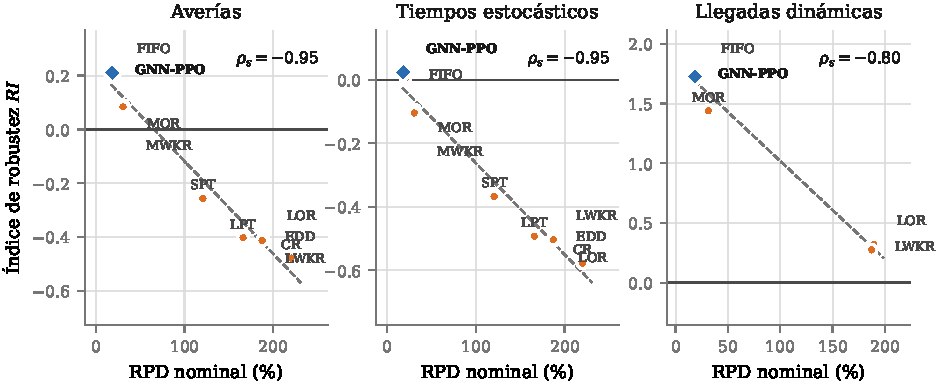
\includegraphics[width=\textwidth]{figures/Fig1_ri_artifact}
  \caption{El índice de robustez frente a la desviación nominal, agregado por
  clase de perturbación. Cada punto es un método. La línea discontinua es un
  ajuste por mínimos cuadrados mostrado solo como orientación; el estadístico
  reportado es la correlación de rangos. Los métodos cuyas planificaciones
  nominales quedan más lejos del óptimo (\textsc{cr}, \textsc{lwkr},
  \textsc{lor}, \textsc{edd}) obtienen los índices más negativos --- es decir,
  convencionalmente, los más robustos.}
  \label{fig:artifact}
\end{figure*}

\NRINeg{} de las \PropCells{} celdas (método $\times$ instancia $\times$ régimen)
del corpus --- el \PctRINeg{}\,\% --- tienen $\RI<0$. Por el Corolario~\ref{cor:neg} cada una es un caso en que
el makespan perturbado esperado está por debajo del nominal, y verificamos que
la equivalencia se cumple exactamente: en el $100\%$ de las celdas,
$\operatorname{signo}(\RI)$ coincide con $\operatorname{signo}(q-r)$. La regla de
razón crítica sobre \texttt{ft06} con $A_k=0{,}90$ es representativa: su
makespan nominal de $171$ cae a una media de $94{,}1$ bajo averías. La regla
calcula una razón de criticidad a partir de fechas de entrega sintetizadas una
sola vez contra duraciones nominales y jamás recalculadas conforme avanza el
reloj realizado, de modo que bajo perturbación sus decisiones de ordenamiento se
vuelven progresivamente menos relacionadas con el estado que ordenan; el
reordenamiento casi aleatorio resultante mejora una secuencia que estaba mal
elegida desde el principio. Esto es regresión a la media, y el índice lo
registra como resiliencia.

\subsection{Inversión de orden y el costo de actuar según ella}
\label{sec:res-reversal}

Si el índice se limitara a añadir ruido, seguiría siendo utilizable en
esperanza. No lo hace: induce un ordenamiento sistemáticamente opuesto al orden
por calidad realizada.

\begin{table*}[t]
\caption{Desacuerdo entre los dos ordenamientos. $\tau$ es la correlación de rangos de Kendall entre el orden por $\RI$ y el orden por calidad realizada. Las tres últimas columnas dan la calidad realizada del método que nomina el índice, la del método realmente mejor, y la penalización de seguir al índice.}\label{tbl:reversal}
\begin{tabular*}{\tblwidth}{@{}LLrllrrr@{}}
\toprule
\multirow{2}{*}{Clase} & \multirow{2}{*}{Severidad} & \multirow{2}{*}{$\tau$} & \multicolumn{2}{c}{Método elegido} & \multicolumn{3}{c}{Calidad realizada (\%)} \\
\cmidrule(lr){4-5}\cmidrule(l){6-8}
 & & & por $\RI$ & por $\RQ$ & del 1.\textordmasculine{} & del 2.\textordmasculine{} & penaliz. \\
\midrule
Averías & $A_k=0.95$ & $-0.600$ & CR & MWKR & 46.9 & 23.6 & $+23.3$ \\
 & $A_k=0.90$ & $-0.422$ & CR & MWKR & 63.3 & 34.8 & $+28.5$ \\
 & $A_k=0.80$ & $-0.511$ & CR & \textbf{GNN--PPO} & 90.6 & 64.9 & $+25.7$ \\
Tiempos estocásticos & $\sigma=0.10$ & $-0.289$ & CR & MWKR & 30.6 & 12.3 & $+18.4$ \\
 & $\sigma=0.25$ & $-0.378$ & CR & MWKR & 33.7 & 13.7 & $+20.0$ \\
 & $\sigma=0.50$ & $-0.511$ & CR & MWKR & 40.8 & 24.9 & $+15.8$ \\
Llegadas dinámicas & $\rho=0.70$ & $-0.400$ & LWKR & \textbf{GNN--PPO} & 268.0 & 230.4 & $+37.6$ \\
 & $\rho=0.85$ & $-0.600$ & LWKR & \textbf{GNN--PPO} & 268.1 & 219.2 & $+48.9$ \\
 & $\rho=0.95$ & $-0.400$ & LWKR & \textbf{GNN--PPO} & 261.1 & 211.7 & $+49.3$ \\
\bottomrule
\end{tabular*}
\end{table*}


El $\tau$ de Kendall es negativo en los \NRegimes{} regímenes
(Tabla~\ref{tbl:reversal}, rango \TauMin{} a \TauMax{}), y los dos criterios
nunca eligen el mismo método. Las pruebas individuales de $\tau$ por régimen
resultan significativas solo en una minoría --- con diez métodos como máximo por
régimen tienen poca potencia ---, pero el signo es negativo sin excepción, y es
la consistencia de ese signo a lo largo de nueve regímenes independientes, y no
ningún valor $p$ aislado, lo que sostiene la afirmación. El índice elige la regla de razón crítica en los
\CRWins{} regímenes de averías y tiempos estocásticos, y menor trabajo restante
en los \LWKRWins{} de llegadas. La calidad realizada elige mayor trabajo
restante o la política aprendida. La penalización por seguir al índice --- la
diferencia en calidad realizada entre el método que nomina y el que realmente es
mejor --- va de \PenaltyMin{} a \PenaltyMax{} puntos porcentuales, con mediana
\PenaltyMedian{}. La Figura~\ref{fig:reversal} muestra la inversión de forma
directa.

\begin{figure*}[t]
  \centering
  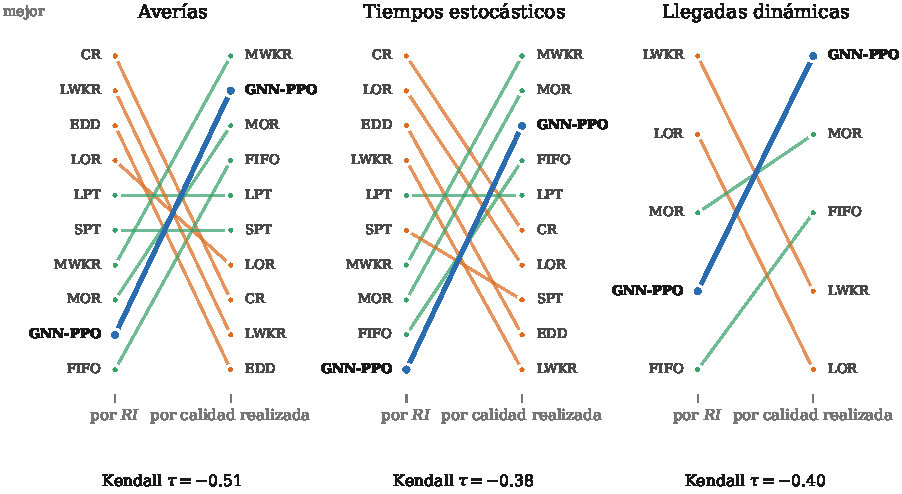
\includegraphics[width=\textwidth]{figures/Fig2_rank_reversal}
  \caption{Ordenamiento por el índice de robustez (izquierda) frente al
  ordenamiento por calidad realizada (derecha), por clase de perturbación. Las
  líneas que descienden de izquierda a derecha corresponden a métodos que el
  índice favorece indebidamente. La política aprendida viaja de casi la peor
  posición a la mejor; las reglas de fecha de entrega viajan en sentido
  contrario.}
  \label{fig:reversal}
\end{figure*}

\subsection{Calidad realizada y riesgo de cola}\label{sec:res-rq}

La Tabla~\ref{tbl:axis} da el panel completo de métricas. Leer las columnas unas
contra otras es instructivo: el orden de la columna $\RI$ se aproxima al inverso
del orden de la columna $\RQ$, y la columna de desviación nominal explica el
primero casi por completo.

\begin{table}[t]
\caption{Panel de métricas por clase de perturbación, métodos ordenados por calidad realizada. $r$ es la desviación nominal respecto del óptimo certificado; $\RI$ el índice convencional; $\RQ$ la calidad realizada; $\CVaR_{90}$ la media de su peor decil. Todos en porcentaje. $^{\star}$ marca la política aprendida.}\label{tbl:axis}
\begin{tabular*}{\tblwidth}{@{}Lrrrr@{}}
\toprule
Método & $r$ (\%) & $\RI$ & $\RQ$ (\%) & $\CVaR_{90}$ (\%) \\
\midrule
\multicolumn{5}{@{}l}{\textit{Averías}} \\[2pt]
\quad MWKR & 30.7 & +0.084 & 41.7 & 88.0 \\
\quad \textbf{GNN--PPO}$^{\star}$ & 18.4 & +0.210 & 41.8 & 85.3 \\
\quad MOR & 31.5 & +0.090 & 43.2 & 85.6 \\
\quad FIFO & 21.1 & +0.212 & 46.8 & 89.6 \\
\quad LPT & 165.9 & -0.402 & 57.7 & 107.4 \\
\quad SPT & 120.7 & -0.256 & 64.2 & 122.8 \\
\quad LOR & 189.2 & -0.410 & 65.8 & 130.3 \\
\quad CR & 220.1 & -0.478 & 67.0 & 131.1 \\
\quad LWKR & 187.4 & -0.412 & 68.8 & 134.6 \\
\quad EDD & 187.4 & -0.411 & 69.2 & 129.7 \\
\addlinespace
\multicolumn{5}{@{}l}{\textit{Tiempos estocásticos}} \\[2pt]
\quad MWKR & 30.7 & -0.105 & 17.0 & 36.0 \\
\quad MOR & 31.5 & -0.094 & 19.1 & 38.0 \\
\quad \textbf{GNN--PPO}$^{\star}$ & 18.4 & +0.023 & 20.0 & 43.4 \\
\quad FIFO & 21.1 & +0.006 & 21.9 & 49.4 \\
\quad LPT & 165.9 & -0.493 & 33.2 & 59.8 \\
\quad CR & 220.1 & -0.578 & 35.0 & 67.0 \\
\quad LOR & 189.2 & -0.505 & 38.6 & 69.8 \\
\quad SPT & 120.7 & -0.368 & 39.6 & 63.8 \\
\quad EDD & 187.4 & -0.505 & 42.2 & 71.4 \\
\quad LWKR & 187.4 & -0.503 & 42.6 & 74.6 \\
\addlinespace
\multicolumn{5}{@{}l}{\textit{Llegadas dinámicas}} \\[2pt]
\quad \textbf{GNN--PPO}$^{\star}$ & 18.4 & +1.728 & 220.4 & 275.1 \\
\quad MOR & 31.5 & +1.441 & 221.1 & 273.4 \\
\quad FIFO & 21.1 & +1.762 & 234.7 & 287.1 \\
\quad LWKR & 187.4 & +0.275 & 265.7 & 307.6 \\
\quad LOR & 189.2 & +0.321 & 266.4 & 310.6 \\
\bottomrule
\end{tabular*}
\end{table}


Bajo averías la política aprendida alcanza $\RQ=41{,}8\%$ con
$\CVaR_{90}=85{,}3\%$ --- la mejor cola del panel --- mientras que \textsc{mwkr}
alcanza una media marginalmente mejor ($41{,}7\%$) con peor cola ($88{,}0\%$).
La regla de razón crítica, que el índice convencional sitúa primera, realiza
$67{,}0\%$ con una cola de $131{,}1\%$. Bajo tiempos de proceso estocásticos
\textsc{mwkr} lidera en media y en cola, con la política en tercer lugar. Bajo
llegadas dinámicas la política lidera en media y \textsc{mor} en cola, ambas
próximas; las magnitudes absolutas en esta clase son grandes por la razón dada
en la Sección~\ref{sec:framework} y deben leerse comparativamente. La
Figura~\ref{fig:rq} muestra media y cola conjuntamente.

\begin{figure*}[t]
  \centering
  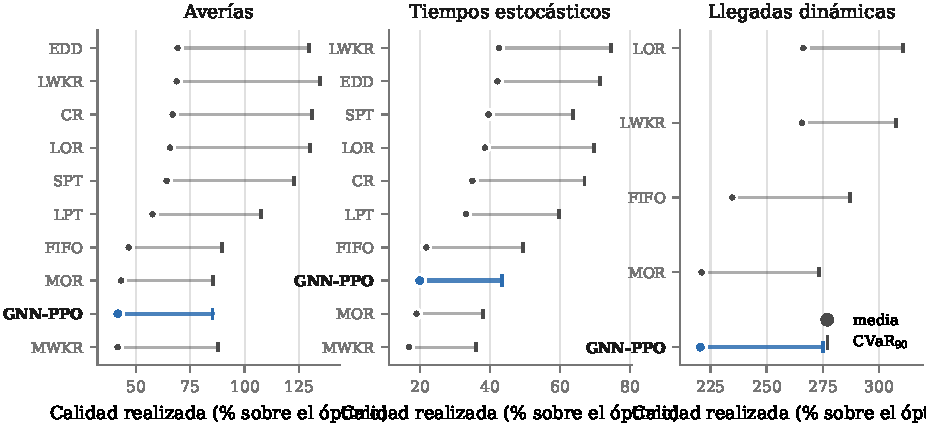
\includegraphics[width=\textwidth]{figures/Fig4_realized_quality}
  \caption{Calidad realizada por método y clase de perturbación. El círculo es
  la media, la marca vertical el $\CVaR_{90}$, y el segmento entre ambos la
  exposición de cola. Los métodos están ordenados por calidad realizada media.}
  \label{fig:rq}
\end{figure*}

\subsection{Separación de métodos bajo la métrica corregida}
\label{sec:res-friedman}

\begin{table*}[t]
\caption{Pruebas de Friedman sobre calidad realizada con post-hoc de Nemenyi, por régimen. Los bloques son pares (instancia, semilla). La última columna indica si la política aprendida es estadísticamente indistinguible del método mejor clasificado a la diferencia crítica.}\label{tbl:friedman}
\begin{tabular*}{\tblwidth}{@{}LLrrrlrlrc@{}}
\toprule
Clase & Severidad & $k$ & $N$ & $\chi^2$ & $p$ & CD & Mejor rango & Rango GNN--PPO & Empata \\
\midrule
Averías & $A_k=0.95$ & 10 & 60 & 256.0 & $<10^{-8}$ & 1.75 & MWKR & 2.83 & \checkmark \\
 & $A_k=0.90$ & 10 & 60 & 252.5 & $<10^{-8}$ & 1.75 & \textbf{GNN--PPO} & 2.83 & \checkmark \\
 & $A_k=0.80$ & 10 & 60 & 170.4 & $<10^{-8}$ & 1.75 & \textbf{GNN--PPO} & 3.12 & \checkmark \\
Tiempos estocásticos & $\sigma=0.10$ & 10 & 60 & 289.1 & $<10^{-8}$ & 1.75 & MWKR & 3.28 & \checkmark \\
 & $\sigma=0.25$ & 10 & 60 & 267.3 & $<10^{-8}$ & 1.75 & MWKR & 3.15 & \checkmark \\
 & $\sigma=0.50$ & 10 & 60 & 150.6 & $<10^{-8}$ & 1.75 & MWKR & 3.85 & \checkmark \\
Llegadas dinámicas & $\rho=0.70$ & 5 & 60 & 183.0 & $<10^{-8}$ & 0.79 & \textbf{GNN--PPO} & 1.62 & \checkmark \\
 & $\rho=0.85$ & 5 & 60 & 200.4 & $<10^{-8}$ & 0.79 & \textbf{GNN--PPO} & 1.57 & \checkmark \\
 & $\rho=0.95$ & 5 & 60 & 190.1 & $<10^{-8}$ & 0.79 & \textbf{GNN--PPO} & 1.57 & \checkmark \\
\bottomrule
\end{tabular*}
\end{table*}


La hipótesis nula de Friedman se rechaza en todos los regímenes con
$p\le\FriedmanPMax{}$ (Tabla~\ref{tbl:friedman}), de modo que los métodos son
distinguibles en calidad realizada en todas partes. La política aprendida es el
método mejor clasificado en \NRLBest{} de \NRegimes{} regímenes y no es
significativamente peor que el mejor clasificado en ninguno de los
\NRLNotWorse{}.

Bajo llegadas dinámicas la política ocupa el primer rango en los tres regímenes,
con rangos promedio de \ArrRankMin{}--\ArrRankMax{} frente a una diferencia
crítica de \ArrCD{}. No queda, sin embargo, separada de todo el campo:
\textsc{mor} la sigue por apenas \ArrGapMin{}--\ArrGapMax{} puntos de rango,
holgadamente dentro de la diferencia crítica, de modo que el enunciado correcto
es que la política y \textsc{mor} empatan estadísticamente en la cima mientras
\textsc{fifo}, \textsc{lwkr} y \textsc{lor} quedan fuera. La
Figura~\ref{fig:cd} muestra los diagramas de diferencia crítica, en los que la
barra de camarilla abarca exactamente ese par. La misma lectura aplica en los
otros seis regímenes, donde la camarilla de la política contiene además a
\textsc{mwkr}, \textsc{mor} y \textsc{fifo}: en ningún punto de este corpus la
política aprendida se separa de todas las reglas.

\begin{figure*}[t]
  \centering
  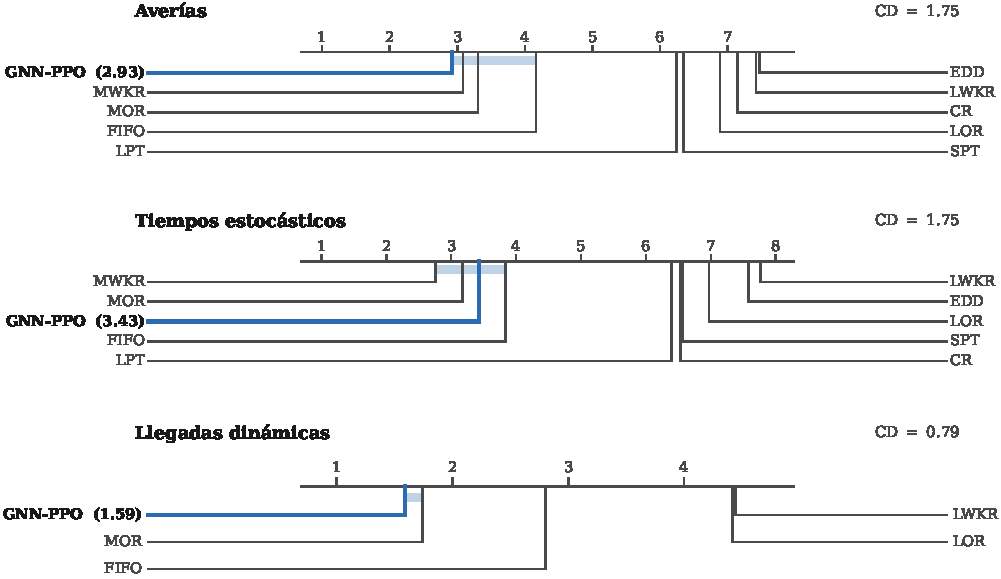
\includegraphics[width=\textwidth]{figures/Fig3_critical_difference}
  \caption{Diagramas de diferencia crítica sobre calidad realizada, uno por
  clase de perturbación. Los métodos unidos por la barra sombreada no son
  distinguibles del mejor clasificado con $\alpha=0{,}05$.}
  \label{fig:cd}
\end{figure*}

\subsection{Sensibilidad al comparador}\label{sec:res-comparators}

La Tabla~\ref{tbl:comparators} evalúa los tres comparadores de la
Sección~\ref{sec:comparators} sobre el corpus nominal de \NInstances{}
instancias.

\begin{table*}[t]
\caption{La misma política frente a tres definiciones de «mejor regla de despacho». Las desviaciones son RPD respecto del óptimo certificado; la columna de diferencia es la mediana de la diferencia pareada en puntos porcentuales, con $z$, $p$ de Wilcoxon y tamaño de efecto biserial de rangos sobre las instancias pareadas; $N=43$ en las filas de la política aprendida y $N=40$ donde se descartan empates exactos, como registra la columna $n$.}\label{tbl:comparators}
\begin{tabular*}{\tblwidth}{@{}LrLrrrrlrl@{}}
\toprule
Comparador & Su RPD & Método & Su RPD & Dif.\ mediana & $n$ & $z$ & $p$ & $r_{rb}$ & Veredicto \\
\midrule
$\mathrm{PDR}_{\mathrm{global}}$ & 251.4 & \textbf{GNN--PPO} & 24.8 & $+233.4$ & 43 & -5.71 & $1.1\times10^{-8}$ & $+1.000$ & \textsc{gana} \\
 & 251.4 & GA & 5.5 & $+251.5$ & 43 & -5.71 & $1.1\times10^{-8}$ & $+1.000$ & \textsc{gana} \\
 & 251.4 & CP-SAT & 0.0 & $+254.6$ & 43 & -5.71 & $1.1\times10^{-8}$ & $+1.000$ & \textsc{gana} \\
$\mathrm{PDR}_{\mathrm{family}}$ & 148.1 & \textbf{GNN--PPO} & 24.8 & $+132.4$ & 43 & -5.71 & $1.1\times10^{-8}$ & $+1.000$ & \textsc{gana} \\
 & 148.1 & GA & 5.5 & $+144.3$ & 43 & -5.71 & $1.1\times10^{-8}$ & $+1.000$ & \textsc{gana} \\
 & 148.1 & CP-SAT & 0.0 & $+152.1$ & 43 & -5.71 & $1.1\times10^{-8}$ & $+1.000$ & \textsc{gana} \\
$\mathrm{PDR}_{\mathrm{oracle}}$ & 19.0 & \textbf{GNN--PPO} & 24.8 & $-7.6$ & 43 & -4.11 & $4.0\times10^{-5}$ & $-0.719$ & \textsc{pierde} \\
 & 19.0 & GA & 5.5 & $+11.5$ & 40 & -5.51 & $3.6\times10^{-8}$ & $+1.000$ & \textsc{gana} \\
 & 19.0 & CP-SAT & 0.0 & $+21.1$ & 40 & -5.51 & $3.6\times10^{-8}$ & $+1.000$ & \textsc{gana} \\
\bottomrule
\end{tabular*}
\end{table*}


El veredicto sobre la política aprendida depende por completo del comparador
elegido. Frente a la media de las nueve reglas gana por \CompGlobal{} puntos
porcentuales; frente a la mejor regla por familia, por \CompFamily{}; frente al
oráculo por instancia, \emph{pierde} por \CompOracle{}. Las tres diferencias son
significativas sobre $N=\NInstances{}$ instancias pareadas
($p\le\CompPMax{}$; valores exactos en la Tabla~\ref{tbl:comparators}). Un
trabajo que reportara solo la primera afirmaría una victoria decisiva; uno que
reportara solo la tercera, una derrota decisiva. Ambos estarían describiendo las
mismas corridas. La Figura~\ref{fig:comparators} muestra las tres
distribuciones.

\begin{figure*}[t]
  \centering
  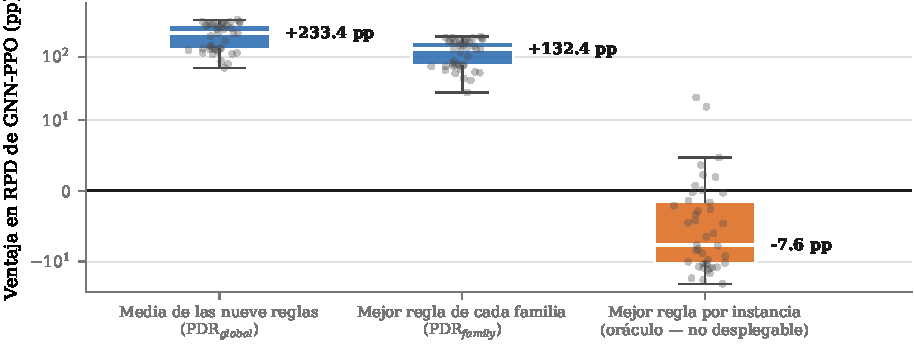
\includegraphics[width=\textwidth]{figures/Fig6_comparator_sensitivity}
  \caption{Ventaja de la política aprendida sobre tres definiciones de la línea
  base de reglas de despacho, por instancia. La escala vertical es
  logarítmica simétrica. El comparador de oráculo se incluye como calibración y
  no es desplegable.}
  \label{fig:comparators}
\end{figure*}

\subsection{Qué compra la optimalidad bajo perturbación}\label{sec:res-exact}

Una comparación complementaria atañe a la afirmación motivadora de la literatura
de programación con DRL. Sobre \texttt{ft06} bajo averías con $A_k=0{,}90$,
tanto CP-SAT como el algoritmo genético alcanzan el óptimo probado en lo nominal
($r=0$). Ejecutados con reparación por desplazamiento a la derecha sobre cinco
semillas de perturbación compartidas, realizan \QCpsat{}\,\% y \QGa{}\,\% por
encima del óptimo respectivamente --- frente a \QMor{}\,\% de \textsc{mor},
\QMwkr{}\,\% de \textsc{mwkr} y \QRl{}\,\% de la política aprendida. Las
diferencias pareadas entre la política y el método exacto o el metaheurístico no
son significativas a este tamaño muestral ($p=\PRlCpsat{}$ y $p=\PRlGa{}$; una
semilla produce un empate exacto para los tres métodos, dejando
$n=\NEffOffline{}$ diferencias no nulas). El algoritmo genético consume
\WallGa{}~s por instancia y CP-SAT \WallCpsat{}~s, frente a \WallRl{}~s del
despliegue completo de la política.

La lectura que extraemos es deliberadamente cautelosa. Cinco semillas sobre una
instancia en un régimen es una observación descriptiva, no una prueba, y así la
reportamos. Lo que sí sugiere es que la optimalidad nominal se disipa en buena
medida con la ejecución por desplazamiento a la derecha, que es la pregunta
sustantiva que el índice de robustez se introdujo para responder y que la
calidad realizada responde de forma directa.

% ===========================================================================
\section{Discusión}\label{sec:discussion}

\subsection{Qué estaba midiendo el índice}

La Proposición~\ref{prop:ri} muestra que $\RI$ es una diferencia normalizada
entre calidad realizada y nominal, y la Sección~\ref{sec:res-artifact} muestra
que en la práctica domina el término nominal. Conviene entonces entender el
índice no como una medida de robustez que resulta ser ruidosa, sino como una
medida de una cantidad distinta --- a grandes rasgos, cuánto margen se dejó a sí
mismo un método --- reportada bajo un nombre que invita a la interpretación
equivocada. Un método sin margen, porque programó bien, no puede puntuar bien en
ella.

Esto no vacía la pregunta subyacente. «¿Cuánto de su calidad planeada retiene un
método bajo realización?» es una pregunta real e importante, y la diferencia
$q-r$ la responde en una escala interpretable. Lo que debe abandonarse es la
normalización por $\Cmax^{\text{nom}}$ y, con ella, la práctica de comparar
$\RI$ entre métodos.

\subsection{Implicaciones para los resultados publicados}

No estamos en posición de reanalizar los datos de otros autores y no hacemos
afirmación alguna sobre la corrección de ningún resultado publicado concreto. Lo
que la Proposición~\ref{prop:ri} sí establece es condicional y, creemos,
consecuente: dondequiera que una comparación de métodos descanse sobre un índice
de la forma de la Definición~\ref{def:ri}, y dondequiera que los métodos
comparados difieran apreciablemente en calidad nominal, el orden reportado queda
confundido por esa diferencia en una dirección conocida y por una magnitud
computable. Dado que las políticas aprendidas y las reglas de despacho difieren
rutinariamente por un factor de varias unidades en desviación nominal --- en
las dos instancias de perturbación de este corpus, \NomRlTwo{}\,\% de la
política aprendida frente a \NomCrTwo{}\,\% de la regla de razón crítica, y
\NomRlAll{}\,\% frente a \NomCrAll{}\,\% sobre el conjunto nominal completo de
\NInstances{} instancias ---, la condición no es un caso límite.

El remedio es barato. La calidad realizada es computable a partir de registros
que cualquier estudio de este tipo ya posee, siempre que exista un óptimo
certificado o una cota aceptada para la instancia nominal; no exige
reejecución. Recomendaríamos reportar $r$, $q$ y $q-r$ juntos, y reservar el
lenguaje de robustez para el tercero.

\subsection{Un protocolo de reporte}

La auditoría sugiere cuatro requisitos, ninguno gravoso.
\begin{enumerate}[(1)]
\item Calificar el desempeño perturbado contra una referencia externa al método:
un óptimo certificado donde exista y, en su defecto, una cota fija compartida
por todos los métodos y nombrada como tal.
\item Reportar la desviación nominal junto a cualquier cantidad de robustez, de
modo que el lector pueda realizar por sí mismo la descomposición de la
Proposición~\ref{prop:ri}.
\item Reportar un estadístico de cola, no solo una media.
\item Nombrar el comparador. Si la afirmación es contra «la mejor regla de
despacho», indicar cuál de las tres construcciones de la
Sección~\ref{sec:comparators} se entiende, y preferir reportar más de una.
\end{enumerate}

\subsection{Amenazas a la validez}\label{sec:threats}

Declaramos los límites de este estudio con franqueza, porque varios acotan las
conclusiones de forma material.

\paragraph{Amplitud de instancias en la malla de perturbación.} Los \NRegimes{}
regímenes se ejecutan sobre dos instancias, \texttt{ft06} y \texttt{la01}. El
resultado analítico de la Proposición~\ref{prop:ri} es independiente de la
instancia, y las correlaciones empíricas se computan entre métodos y no entre
instancias, de modo que la afirmación central de la auditoría no descansa sobre
la amplitud de instancias. Los hallazgos a nivel de método de la
Sección~\ref{sec:res-friedman} sí lo hacen, y deben leerse como válidos para
estas dos instancias y este modelo de perturbación, no como un ordenamiento
general.

\paragraph{Equivalencia a partir de un no rechazo.} Un no rechazo de Nemenyi es
una incapacidad de distinguir, no una demostración de equivalencia. Con $k=10$ y
$N=60$ la diferencia crítica es $1{,}75$ sobre una escala de rangos de $1$ a
$10$, que es amplia; el enunciado de que la política «no es significativamente
peor» debe leerse con esa amplitud en mente y no como afirmación de paridad.

\paragraph{Semillas de entrenamiento.} La política aprendida es un único punto
de control entrenado. Su posición en la Tabla~\ref{tbl:friedman} no lleva por
tanto estimación alguna de la varianza de entrenamiento, y la literatura de
reproducibilidad en aprendizaje por refuerzo es enfática en que esa varianza
puede ser grande \citep{henderson2018,agarwal2021}. La infraestructura de
entrenamiento multisemilla está implementada y documentada en el repositorio
adjunto, pero la campaña multisemilla no había concluido al momento de escribir,
y aquí no se afirma ninguna cifra multisemilla.

\paragraph{Cobertura de métodos bajo perturbación.} La malla de nueve regímenes
compara la política aprendida contra nueve reglas de despacho en seis regímenes
y cuatro en los otros tres (Sección~\ref{sec:execution}). CP-SAT y el algoritmo
genético entran solo por la comparación descriptiva de la
Sección~\ref{sec:res-exact}, con una instancia, un régimen y cinco semillas. En
consecuencia, dondequiera que este trabajo diga que la política no es
significativamente peor que el mejor método,
el conjunto de comparación son las reglas de despacho de ese régimen y no los
solucionadores exacto y metaheurístico --- y en el único régimen donde estos se
ejecutaron terminan por delante de la política (\QCpsat{}\,\% y \QGa{}\,\%
frente a \QRl{}\,\%), aunque no de forma significativa con
$n=\NEffOffline{}$. Un brazo completo de métodos fuera de línea a lo largo de la
malla es el experimento siguiente natural y convertiría la
Sección~\ref{sec:res-exact} de observación en prueba.

\paragraph{Cobertura de reglas bajo llegadas, y por qué no es conservadora.}
Cinco de los diez métodos se comparan en los regímenes de llegadas, por las
razones dadas en la Sección~\ref{sec:execution}. Esto corta en dos direcciones y
queremos ser explícitos con ambas. Para la afirmación de medición es casi
neutro: el conjunto excluido contiene tanto reglas con planificaciones nominales
el conjunto excluido cubre todo el rango: contiene las dos reglas con las peores
planificaciones nominales (\textsc{cr}, \textsc{edd}) y también la de segunda
mejor (\textsc{mwkr}, con \NomMwkrTwo{}\,\%), de modo que no fabrica la
correlación negativa --- que en todo caso descansa sobre los \NConfRegimes{}
regímenes de diez métodos. Para la afirmación sobre la política aprendida es
\emph{anti}conservador: \textsc{mwkr}, que supera en rango a la política en
cinco de los seis regímenes restantes, queda excluida, de modo que el primer rango de la política bajo
llegadas es un primer rango en un campo debilitado. No tratamos por tanto el
resultado de llegadas como la evidencia más fuerte a favor de la política, y a
un lector que lo descuente por completo le queda el argumento de medición, que
no depende de él.

\paragraph{Validez de la referencia bajo llegadas.} Como se señaló en la
Sección~\ref{sec:framework}, $\RQ$ bajo llegadas dinámicas está referenciada al
óptimo de la instancia nominal y no al de la realizada. Las comparaciones dentro
de un régimen siguen siendo válidas; las magnitudes absolutas allí no son
brechas de optimalidad.

\paragraph{Carácter posterior de la remedición.} La auditoría de medición no fue
preregistrada. La motivó un examen de la métrica y se reporta como análisis
posterior de un corpus congelado. No se alteró dato alguno, y los veredictos
preregistrados computados sobre la métrica original permanecen tal como quedaron
registrados en los materiales adjuntos.

% ===========================================================================
\section{Conclusión}\label{sec:conclusion}

El índice de robustez que domina la evaluación de la programación dinámica bajo
perturbación normaliza la degradación de un método por su propio makespan
nominal. Demostramos que ello lo vuelve estrictamente decreciente en la
desviación nominal a desempeño realizado fijo, de modo que cuanto peor es el
plan de un método más robusto parece, y que un índice negativo --- leído
ampliamente como resiliencia excepcional --- es la firma de un plan lo bastante
deficiente como para que la perturbación lo mejore. En un corpus preregistrado
de \NRunsDisrupted{} ejecuciones perturbadas en \NRegimes{} regímenes, el índice
correlaciona por rangos de forma negativa con la desviación nominal en todas
partes, y con $\rho_s\in[\RhoConfMin{},\RhoConfMax{}]$ en los \NConfRegimes{}
regímenes de campo completo, ordena los métodos de forma opuesta a la calidad
realizada en todos los regímenes, y seguirlo cuesta hasta \PenaltyMax{} puntos
porcentuales de desviación respecto del óptimo.

La calidad realizada --- la desviación del makespan ejecutado respecto de un
óptimo certificado --- junto con una cola $\CVaR_{90}$ y un comparador de
despacho explícitamente nombrado, repara la comparación al costo de una simple
remedición. Remedida así, la política GNN--PPO heterogénea no es
significativamente peor que la mejor regla de despacho en ninguno de los
\NRegimes{} regímenes y ocupa el primer rango en \NRLBest{}, incluidos los tres
de llegadas dinámicas, donde el valor de decidir en línea es mayor --- en todos
los casos empatada con \CliqueArr{} regla bajo llegadas y \CliqueOther{} en el
resto, antes que separada del campo. El índice
convencional sitúa a esa misma política cerca del fondo de esas mismas corridas.

El punto más amplio es metodológico. Una métrica cuyo denominador lo elige el
método que se califica no puede sostener una comparación entre métodos, y la
literatura de programación dispone de una referencia externa bien establecida en
los óptimos certificados de sus bancos de prueba estándar. Usarla no cuesta nada
y zanja la pregunta que el índice se introdujo para responder.

% ===========================================================================
\section*{Declaración de contribución de autoría CRediT}

\textbf{Joseph Javier Sánchez Acuña:} Conceptualización, Metodología, Software,
Análisis formal, Investigación, Curación de datos, Redacción -- borrador
original, Redacción -- revisión y edición, Visualización.

\section*{Declaración de intereses en competencia}

El autor declara no tener intereses financieros ni relaciones personales
conocidas que pudieran haber influido en el trabajo aquí reportado.

\section*{Disponibilidad de datos}

El código fuente, el documento de preregistro, los registros crudos por corrida
que sustentan cada tabla y figura, y los scripts de análisis que los regeneran
están disponibles en el repositorio público adjunto. Cada cifra reportada en la
Sección~\ref{sec:results}, incluida la auditoría de la identidad de la
Sección~\ref{sec:framework} y la comparación de métodos fuera de línea de la
Sección~\ref{sec:res-exact}, es producida por esos scripts a partir de esos
registros.

\appendix

\section{Programa de investigación}\label{app:gantt}

La Figura~\ref{fig:gantt} expone el cronograma del programa de investigación del
que surge el corpus, incluido el punto en que se congeló el preregistro y aquel
en que se cerró la campaña confirmatoria. La auditoría de medición reportada en
este trabajo es posterior a ambos.

\begin{figure*}[t]
  \centering
  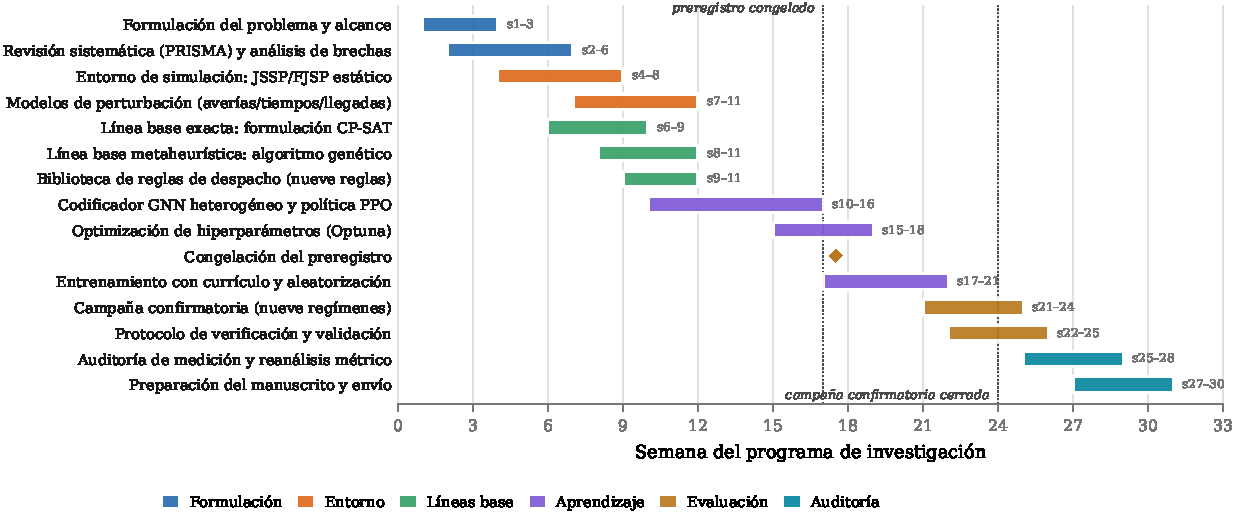
\includegraphics[width=\textwidth]{figures/Fig5_gantt}
  \caption{Cronograma del programa de investigación. El rombo marca la
  congelación del preregistro, tras la cual no se alteró hipótesis, umbral,
  conjunto de instancias ni prueba estadística alguna. La auditoría de medición
  y el reanálisis aquí reportados ocupan la fase final y son posteriores a esa
  congelación.}
  \label{fig:gantt}
\end{figure*}

\printcredits

\bibliographystyle{cas-model2-names}
\bibliography{refs}

\end{document}
